\documentclass[12pt, fleqn]{beamer}
\usepackage[utf8]{inputenc}
\usepackage[T2A]{fontenc}
\usepackage{amssymb, amsmath, mathrsfs, amsthm}
\usepackage[russian]{babel}
\usepackage{graphicx}
\usepackage{indentfirst}
\usepackage{algorithm}
\usepackage{algpseudocode}
\usetheme{Warsaw}
%\addto\captionsrussian{\renewcommand{\figurename}{Рисунок}}
\title{Методы аугментации аудиоданных}
\author{Лукьянов Павел Александрович}
\institute {\normalsize
Научный руководитель: \\
д.ф-м.н., профессор\\
Дьяконов Александр Геннадьевич \normalsize
}
\date{Москва, 2022} 
\begin{document}% начало презентации
	
\begin{frame}
	\titlepage
\end{frame}

\begin{frame}{Аугментация аудиоданных}
	\begin{figure}[h]
		\centering
		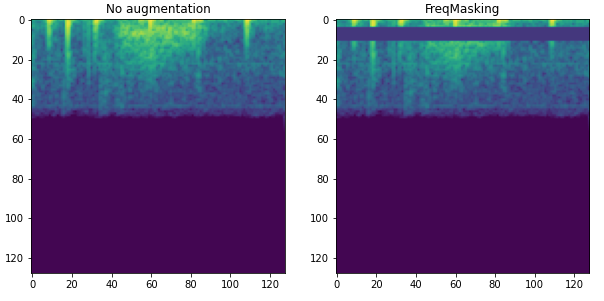
\includegraphics[scale=0.7]{6_0.png}
		\caption{FreqMasking}
		\label{ris:image4}
	\end{figure}
\end{frame}

\begin{frame}{SwapVerticalStripes}
	$T$ --- параметр метода. \newline В результате применения аугментации: 
\begin{enumerate}
    \item $t \sim U\{0, T\}, t_1 \sim U\{t, \text{TimeSize} - 1 - t\}$, \newline $t_2 \sim U\{t, \text{TimeSize} - 1 - t\}, |t_1 - t_2| \geq t.$
    \item $S[:; t_1: t_1 + t - 1] \leftrightarrow S[:; t_2 : t_2 + t - 1]$.
\end{enumerate}
    \begin{figure}[ht!]
    	\center{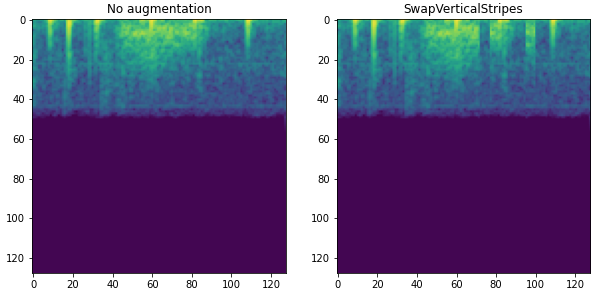
\includegraphics[scale=0.5]{3_0.png}}
    	\caption{SwapVerticalStripes}
    	\label{fig:i3}
    \end{figure}
\end{frame}

\begin{frame}{SwapNeighboringStripes}
	 $T$ --- параметр метода. \newline В результате применения аугментации:
        \begin{enumerate}
            \item $t \sim U\{0, T\}, t_0 \sim U\{t, \text{TimeSize} - 1 - t\}.$
            \item $S[:; t_0: t_0 + t - 1] \leftrightarrow S[:; t_0 - t: t_0 - 1].$
        \end{enumerate}
    \begin{figure}[ht!]
    	\center{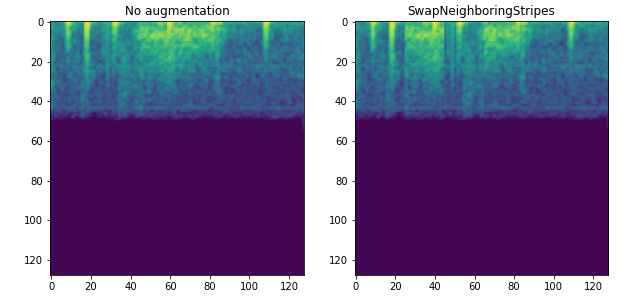
\includegraphics[scale=0.5]{1_0.png}}
    	\caption{SwapNeighboringStripes}
    	\label{fig:i1}
    \end{figure}
\end{frame}

\begin{frame}{SwapSeveralStripes}
     $T, N$ --- параметры метода, $n \sim U\{0, N\}$. \newline
    	В результате применения аугментации (процедура повторяется $n$ раз):
	\begin{enumerate}
        \item $T_0 = \lfloor \frac{T}{n} \rfloor$, $t \sim U\{0, T_0\}, t_1 \sim U\{t, \text{TimeSize} - 1 - t\},$ \newline $t_2 \sim U\{t, \text{TimeSize} - 1 - t\}, |t_1 - t_2| \geq t.$
        \item $S[:; t_1: t_1 + t - 1] \leftrightarrow S[:; t_2 : t_2 + t - 1]$.
       \end{enumerate}
    \begin{figure}[ht!]
    	\center{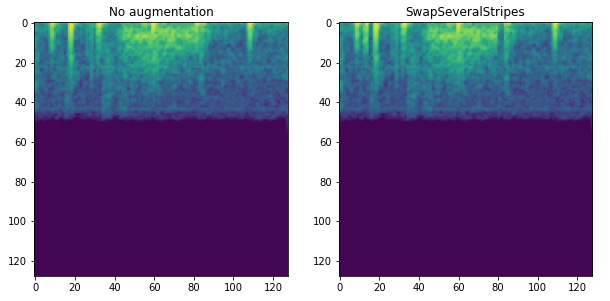
\includegraphics[scale=0.5]{2_0.png}}
    	\caption{SwapSeveralStripes}
    	\label{fig:i2}
    \end{figure}
\end{frame}

\begin{frame}{Эксперименты}
	\begin{table}[ht!]
    \centering
	\begin{tabular}{| l | l | c |}
    	\hline
	    Метод аугментации & resnet18 & resnet50 \\ \hline
	    Аугментация отсутствует  & 81.98 $\pm$ 2.34 & 82.23 $\pm$ 2.4 \\ \hline
	    SwapVerticalStripes & \textbf{83.2 $\pm$ 1.3} & \textbf{83.65 $\pm$ 1.07} \\ \hline
	    SwapNeighboringStripes & 81.62 $\pm$ 0.69 & \textbf{83.4 $\pm$ 1.71} \\ \hline
	    SwapSeveralStripes & \textbf{83.55 $\pm$ 0.49} & \textbf{84.42 $\pm$ 1.92} \\ \hline
	\end{tabular}
	\caption{Результаты экспериментов (Heartbeat Sounds) с предлагаемыми методами аугментации SwapVerticalStripes, SwapNeighboringStripes, SwapSeveralStripes. Метрика качества --- процент верно классифицированных объектов.}
	\label{table:lukianov_pavel_t1}
    \end{table}
\end{frame}

\begin{frame}{Эксперименты}
\begin{table}[ht!]
	\centering
	\begin{tabular}{| l | l | c |}
    	\hline
	    Метод аугментации & resnet18 & resnet50 \\ \hline
	    Аугментация отсутствует  & 0.66 $\pm$ 0.034 & 0.692 $\pm$ 0.04 \\ \hline
	    SwapVerticalStripes & \textbf{0.699 $\pm$ 0.029} & 0.681 $\pm$ 0.038 \\ \hline
	    SwapNeighboringStripes & \textbf{0.69 $\pm$ 0.029} & 0.7 $\pm$ 0.027 \\ \hline
	    SwapSeveralStripes & \textbf{0.687 $\pm$ 0.026} & \textbf{0.709 $\pm$ 0.029} \\ \hline
	\end{tabular}
	\caption{Результаты экспериментов (Heartbeat Sounds) с предлагаемыми методами аугментации SwapVerticalStripes, SwapNeighboringStripes, SwapSeveralStripes. Метрика качества --- сбалансированная точность.}
	\label{table:lukianov_pavel_t1}
\end{table}
\end{frame}

\begin{frame}{Эксперименты}
    \begin{table}[ht!]
    \centering
	\begin{tabular}{| l | l | c |}
    	\hline
	    Метод аугментации & resnet18 & resnet50 \\ \hline
	    Аугментация отсутствует  & 74.3 $\pm$ 3.03 & 73.0 $\pm$ 3.24 \\ \hline
	    SwapVerticalStripes & \textbf{76.6 $\pm$ 2.67} & \textbf{75.6 $\pm$ 3.68} \\ \hline
	    SwapNeighboringStripes & \textbf{75.6 $\pm$ 2.75} & 71.4 $\pm$ 4.91 \\ \hline
	    SwapSeveralStripes & \textbf{75.4 $\pm$ 2.18} & 72.7 $\pm$ 3.4 \\ \hline
	\end{tabular}
	\caption{Результаты экспериментов (GTZAN) с предлагаемыми методами аугментации SwapVerticalStripes, SwapNeighboringStripes, SwapSeveralStripes. Метрика качества --- процент верно классифицированных объектов.}
	\label{table:lukianov_pavel_t2}
\end{table}
\end{frame}

\begin{frame}{Алгоритм применения методов аугментации}

\algrenewcommand\algorithmicdo{\textbf{выполнять}}
\algrenewcommand\algorithmicfor{\textbf{Цикл}}
\algrenewtext{EndFor}{\textbf{Конец цикла}}

\begin{algorithm}[H]
    \caption{Предлагаемый алгоритм}\label{alg:Alg1}
    \begin{algorithmic}
    \State $\text{Augmentations} = \{Augment_1, Augment_2, ..., Augment_n\}$ --- заданный набор аугментаций,
    \State $Augment$ --- случайно выбранная аугментация  из $\text{Augmentations}$,
    \State $(X_{val}, y_{val})$ --- валидационный датасет, 
    \State $(X_{train}, y_{train})$ --- обучающая выборка,
    \State $f$ --- метрика качества,
    \State $M$ --- число эпох обучения нейронной сети.
    \For{\textbf{от} $j=1$ \textbf{до} M}
    \State train-шаг с применением $Augment$,
    \State вычисление $F_i = f(Augment_i(X_{val}), y_{val}), i = \overline{1,n}$,
    \State $Augment = Augment_k$, где $k = argmin_k(F_k)$.
    \EndFor
    \end{algorithmic}
\end{algorithm}
\end{frame}


\begin{frame}{Эксперименты}
	\begin{table}[ht!]
    \centering
	\begin{tabular}{| l | l | c |}
    	\hline
	    Метод аугментации & resnet18 & resnet50 \\ \hline
	    Аугментация отсутствует  & 81.98 $\pm$ 2.34 & 82.23 $\pm$ 2.4 \\ \hline
	    RandAugment & 83.1 $\pm$ 0.92 & 84.57 $\pm$ 1.3 \\ \hline
	    Предлагаемый алгоритм & \textbf{86.65 $\pm$ 0.67} & \textbf{86.75 $\pm$ 0.76} \\ \hline
	\end{tabular}
	\caption{Результаты экспериментов (Heartbeat Sounds) с предлагаемым алгоритмом применения методов аугментации. Метрика качества --- процент верно классифицированных объектов.}
	\label{table:lukianov_pavel_t3}
\end{table}
\end{frame}

\begin{frame}{Эксперименты}
	\begin{table}[ht!]
    \centering
	\begin{tabular}{| l | l | c |}
    	\hline
	    Метод аугментации & resnet18 & resnet50 \\ \hline
	    Аугментация отсутствует  & 0.66 $\pm$ 0.034 & 0.692 $\pm$ 0.04 \\ \hline
	    RandAugment & 0.713 $\pm$ 0.031 & 0.677 $\pm$ 0.036 \\ \hline
	    Предлагаемый алгоритм & \textbf{0.762 $\pm$ 0.023} & \textbf{0.753 $\pm$ 0.02} \\ \hline
	\end{tabular}
	\caption{Результаты экспериментов (Heartbeat Sounds) с предлагаемым алгоритмом применения методов аугментации. Метрика качества --- сбалансированная точность.}
	\label{table:lukianov_pavel_t3}
\end{table}
\end{frame}

\begin{frame}{Эксперименты}
	\begin{table}[ht!]
    \centering
	\begin{tabular}{| l | l | c |}
    	\hline
	    Метод аугментации & resnet18 & resnet50 \\ \hline
	    Аугментация отсутствует  & 74.3 $\pm$ 3.03 & 73.0 $\pm$ 3.24 \\ \hline
	    RandAugment & 75.0 $\pm$ 2.61 & 74.9 $\pm$ 2.63 \\ \hline
	    Предлагаемый алгоритм & \textbf{76.8 $\pm$ 1.75} & 72.2 $\pm$ 2.8 \\ \hline
	\end{tabular}
	\caption{Результаты экспериментов (GTZAN) с предлагаемым алгоритмом применения методов аугментации. Метрика качества --- процент верно классифицированных объектов.}
	\label{table:lukianov_pavel_t4}
\end{table}
\end{frame}

\begin{frame}{Заключение}
	В процессе выполнения работы получены следующие результаты:
	\begin{itemize}
		\item предложен и реализован метод аугментации аудиоданных SwapVerticalStripes, основанный на перестановке вертикальных полос в мел-спектрограмме, а также его модификации SwapNeighboringStripes, SwapSeveralStripes,
		\item проведены вычислительные эксперименты, показывающие возможную применимость предложенного метода SwapVerticalStripes и его модификаций в задаче аудиоклассификации,
	\end{itemize}
\end{frame}

\begin{frame}{Заключение}
	\begin{itemize}
		\item предложен и реализован алгоритм применения методов аугментации аудиоданных с выбором конкретного метода аугментации после каждой эпохи обучения,
		\item проведены вычислительные эксперименты, показывающие существенное преимущество предложенного алгоритма над алгоритмом RandAugment в задаче аудиоклассификации Heartbeat Sounds Classification.
	\end{itemize}
	По результатам работы сделан доклад на международной научной конференции
студентов, аспирантов и молодых ученых «Ломоносов-2022».
\end{frame}
\end{document}